\chapter{Models and Associated Probes For Proton Spin Structure}
\label{ch:modeling_proton_spin}

With the advances made over the last half-century, we have come very close to
obtaining a complete model describing the world around us.  In the realm of
Rapid progress has been made in the last 40 years in the understanding of the
structure of the nucleon. Protons and neutrons make up the majority of the mass
in the visible universe - therefore understanding their nature completely is of
fundamental importance to physics.

In the previous chapter, we discussed in the history behind studying the
structure of matter, leading up to a brief discussion of the contemporary
experiments in proton spin structure. Glaringly, I neglected to discuss the
Relativistic Heavy Ion Collider (RHIC) and the Pioneering High Energy Nuclear
Interaction eXperiment (PHENIX), since I wanted to put the program into a firm
theoretical context in this chapter.

This thesis will discuss the experimental efforts of PHENIX to do something no
other experiment has done - utilize the production of W-Bosons as a direct probe
of proton spin. 

Before we discuss the specifics of this measurement, lets first put proton spin
into a larger context.

\section{Modeling the Proton Structure}

One frequent theme in using particle accelerators to study any kind of nuclear
structure is that we do not ever get to directly look at the innards of a
proton, due to the phenomena of color confinement.

This means that often, we must deal with the process of how partons (quarks,
gluons) fragment and decay after a proton proton collision. Additionally, we
must deal with and account for the scale-variance of the fundamental forces. 

The scale variance of the fundamental forces has large implications for the
strong nuclear force, generally represented by the coupling constant,
$\alpha_S$. This constant scales with distance, and becomes highly
non-perturbative at short distances.

Non perturbative effects are notoriously difficult to include in analytical
models. Additionally, we find that the very structure and distribution of
partons and gluons in the nucleus is a scale-dependent phenomena, that is to
say, if we take measurements at a lower energy, we get a different distribution
of partons and gluons than if we measure at higher energy. This is not to say
that the proton magically changes itself based on energy, but is really more
related to the length scale that we are probing inside of the proton. 

With higher energies, we probe successively shorter length scales. Therefore, to
form a complete picture of proton spin structure, we must probe by scanning over
a broad range of energies (length scales).

Though we generally can analytically deal with writing down models in
perturbative regimes, we cannot simply throw up our hands and give up making
predictions in non-perturbative regimes. To accomplish this, we use a
Factorization Theorem, which provides us a way to mathematically separate an
interaction into perturbative and non-perturbative parts (example,
Figure~\ref{fig:disschematic}). The non-perturbative aspect in the figure (the
X) is often the portion which is experimentally constrained.

\subsection{Structure Functions}

As a note here, for this work on theoretical background of deep inelastic
scattering, I heavily reference Ciprean Gal's clear and coherent introduction to
the subject, published in 2014 (\cite{Gal2014b}), in his thesis describing the
complimentary analysis done at PHENIX at central rapidities.

Given that the proton itself has so far been shown to be a non-perturbative
object, we need a means to model the structure of the interaction when two
protons collide, and generate particles.  Generally, we can calculate a
structure function associated with each hadronic process. The variables we
define to describe the kinematics are (see Figure~\ref{fig:disschematic}):

\begin{gather}
  P \label{eq:P}\\
  Q^2 \equiv -q^2 \label{eq:big_q_sq}\\
    x \equiv { Q^2 \over {2P\cdot q} } \label{eq:x}
\end{gather}

Where $P$  is the total hadron momentum (in our case, the proton's momentum),
$Q^2$ is the energy exchange between the proton and probe lepton, and $x$ is the
fraction of the total proton's momentum carried by the quark scattering with the
lepton. $q$, in Equation~\ref{eq:x} is four-momentum transferred from the lepton
to the quark. 

We can then write down structure functions in terms of these variables. We have:

\begin{gather}
  F_1(x,Q^2) = {1 \over 2}\sum_f e_f^2 \left(q_f(x)+\bar{q}(x)\right)
  \label{eq:f1} \\
  F_2(x,Q^2) = 2xF_1(x,Q^2)\label{eq:f2}
\end{gather}

The subscript, $f$ refers to the quark flavors represented in the structure
functions, with $e_f$ referring to the charge of each quark being summed over
(i.e. ${\pm}{1\over3}$ or ${\pm}{2\over3}$). $q(x)$ refers to the parton
distribution function associated with each quark flavor. 

An integration over the momentum fraction, $x$ of Equation~\ref{eq:f2} and the
gluon structure function $g(x)$ yields the familiar 'valence quark' structure of
the proton, i.e. two up-quarks and one down quark, with remaining quark flavors
$q_h$ summing to zero:

\begin{gather}
	\int_0^1 F_2(x,Q^2) + g(x) dx 
	= \int_0^1 
	\left(
		x\sum_f e_f^2 \left(q_f(x)+\bar{q}(x)\right) 
	\right) 
	+ g(x) dx \label{eq:f2_int_1} \\
	\int_0^1 \left(u(x)+\bar{u}(x) dx \right) dx = 2  \label{eq:up_quark_valence} \\
	\int_0^1 \left(d(x)+\bar{d}(x) dx \right) dx = 1  \label{eq:down_quark_valence} \\
	\int_0^1 \left(q_h(x)+\bar{q}_h(x) dx \right) dx = 0 \label{eq:other_quark_valence}
\end{gather}

The rest of the world data on $F_2(x,Q^2)$ is summarized in
Figure~\ref{fig:f2_world_data}

\begin{figure}
  \centering
  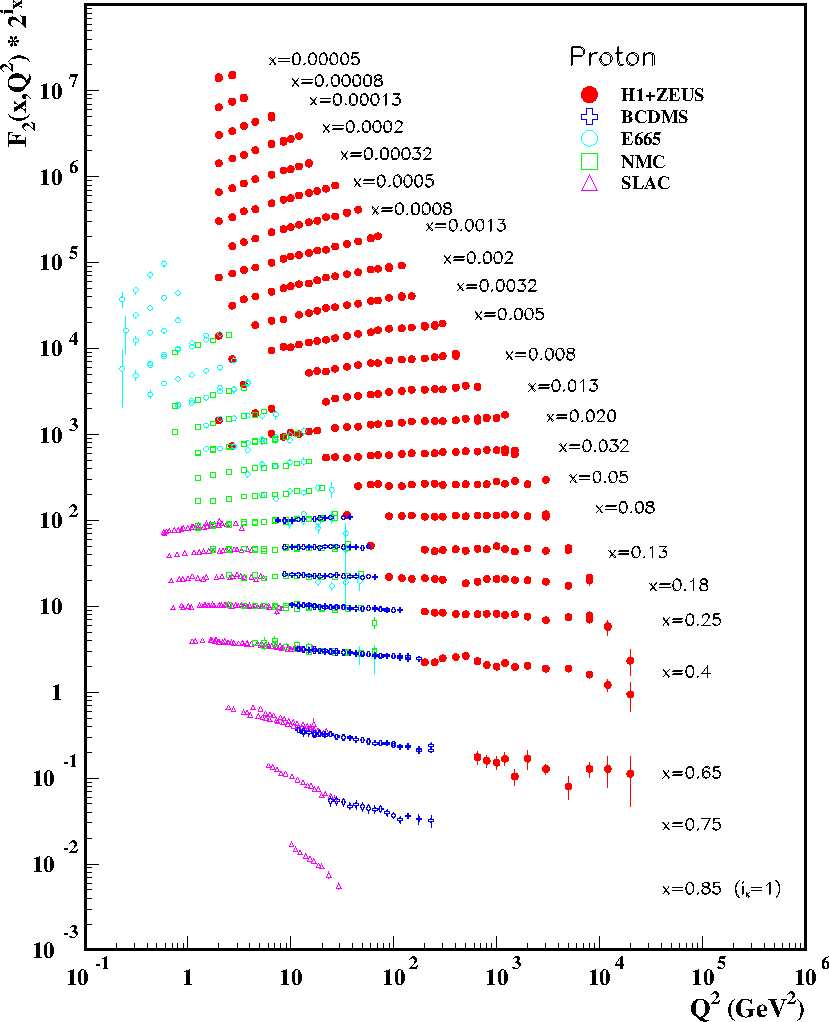
\includegraphics[width=\linewidth]{./figures/F2_structure_function.pdf}
  \caption{
		Here, we see "the proton structure function, $F_2^p$ measured in
		electromagnetic scattering experiments of electrons and positrons on
		protons" from experiments including H1+Zeus, BCDMS, E665, NMC and
		SLAC~\cite{ReviewEidelman2012}
  }
  \label{fig:f2_world_data}
\end{figure}

From this dataset, we can extract Parton Distribution Functions for any
combination of $x$ and $Q^2$. Under this particular framework, we can use the
DGLAP evolution equations to evolve PDFs observed at one $Q^2$ to some other
$Q^2$~\cite{Altarelli2009}. One particular advantage of hadron colliers is to
measure the interactions between gluons and partons between two colliding
partons. 

With QCD evolution, one can additionally undertake a global analysis, which
effectively puts a constraint on Parton Distribution functions using 'evolved
projections' of $x$ and $Q^2$ into the kinematic range of the experimental
probes. 

\section{Parton Distribution Functions}

\begin{figure}[ht]
  \centering
  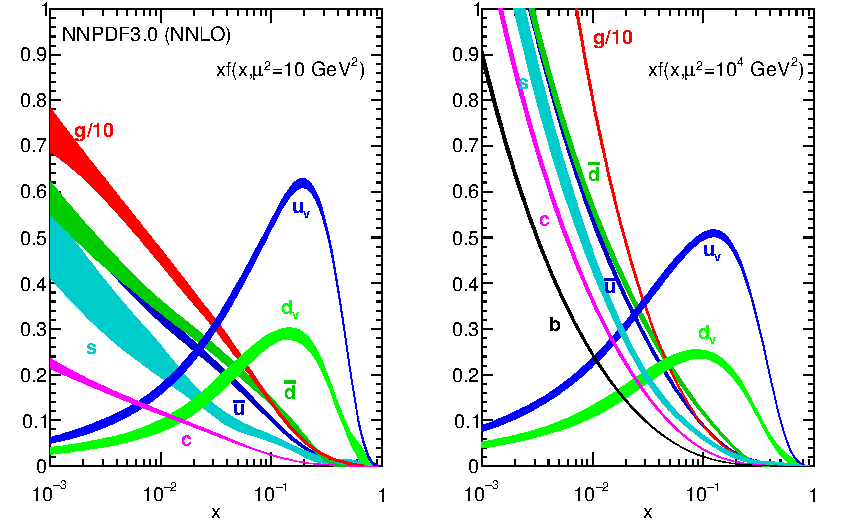
\includegraphics[width=0.7\linewidth]{./figures/unpolarized_pdfs.pdf}
  \caption{
    stuff~\cite{ReviewEidelman2012}
  } 
  \label{fig:unpolarized_pdf}
\end{figure}

\section{Polarized Parton Distribution Functions}
\label{sec:polarized_pdfs}

\begin{figure}
  \centering
  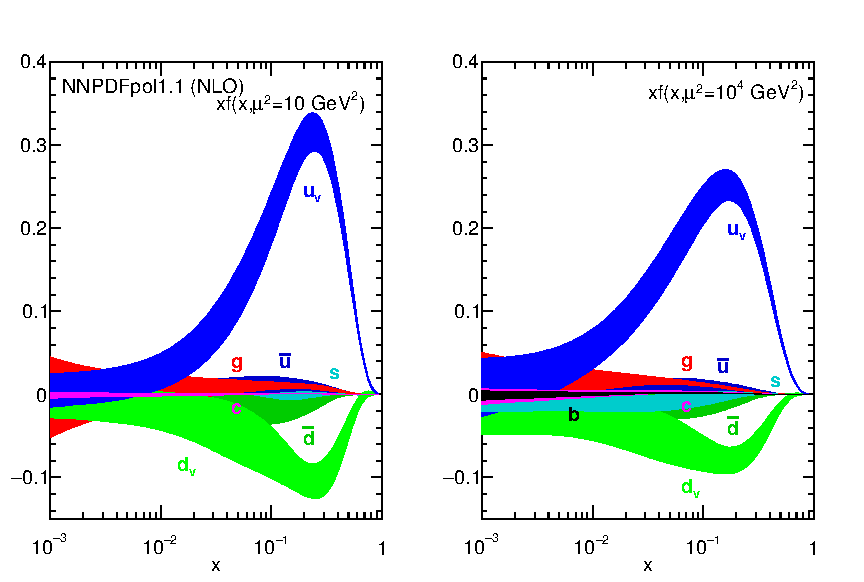
\includegraphics[width=0.7\linewidth]{./figures/polarized_pdfs.pdf}
  \caption{
    stuff~\cite{ReviewEidelman2012}
  }
  \label{fig:polarized_pdfs}
\end{figure}

Discuss DSSV fits
\begin{figure}
  \centering
  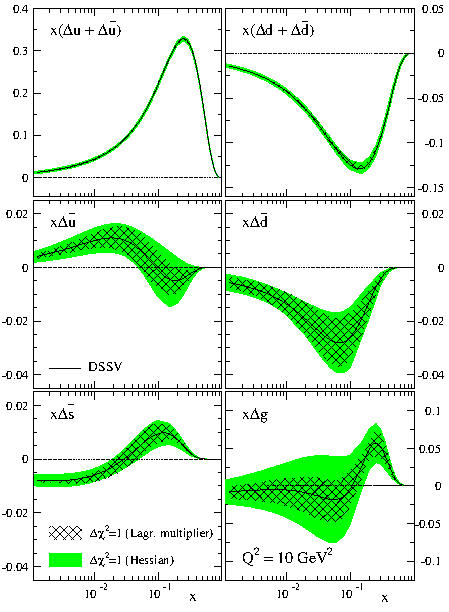
\includegraphics[width=\linewidth]{./figures/polarized_pdfs_dssv.pdf}
  \caption{
    stuff    
  }
  \label{fig:dssv_pdfs}
\end{figure}

\section{Proton Spin Decomposition with the Ellis-Jeffe Sum Rule }

{\noindent}Gauge invariant Ellis-Jeffe
\begin{equation}
  \braket{P,{1\over2}|\hat{J_z}|P,{1\over2}}  
 = {1\over2} = {{1\over2}\Delta \Sigma +L_q+J_g}
\label{eq:ellis_jeffe_sum}
\end{equation}

{\noindent}Infinite momentum decomposition:
\begin{equation}
  \braket{P,{1\over2}|\hat{J_z}|P,{1\over2}}  
  = {1\over2} = {{1\over2}\Delta \Sigma +L_q+\Delta g + L_g}
  \label{eq:infmom_ellis_jeffe_sum}
\end{equation}

{\noindent}Quark decomposition:
\begin{equation}
  {\Delta \Sigma} =
  {
    (\Delta u+\Delta \bar{u})
    +(\Delta d + \Delta \bar{d})
    +(\Delta s + \Delta \bar{s})
  }
  \label{eq:quark_spin_decomposition}
\end{equation}

\section{The Spin Asymmetry: An Experimental Probe }
Write in terms of the cross-section of polarized scattering.

\begin{figure}[ht]
  \centering
  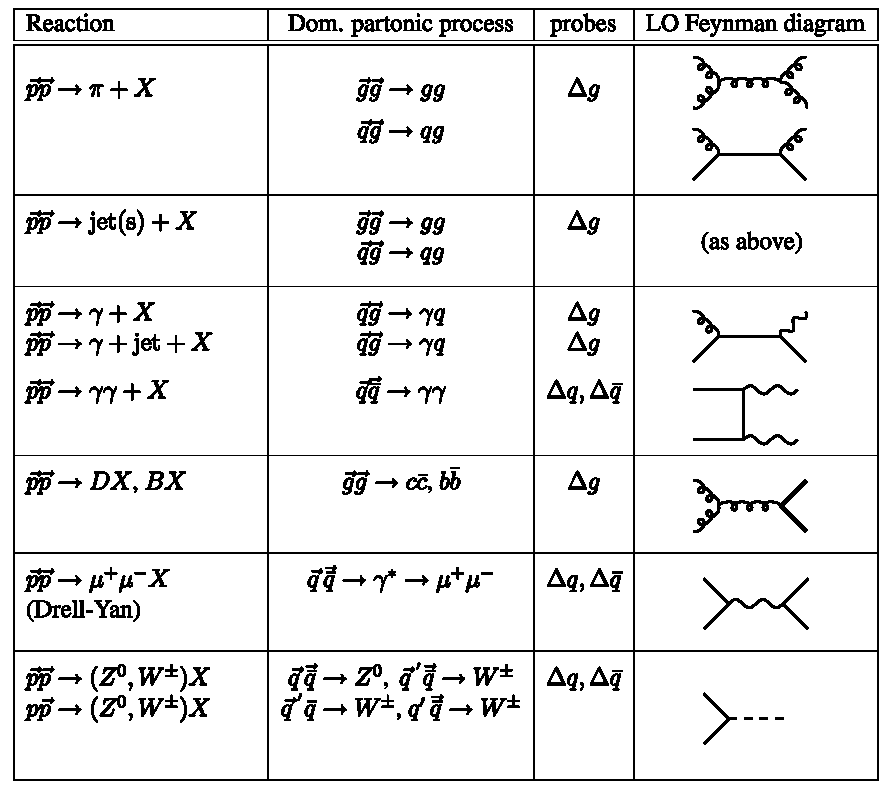
\includegraphics[width=\linewidth]{./figures/spin_probes.pdf}
  \caption{
    A summary of the various probes for longitudinally polarized protons. The
    \textbf{"Reaction"} column summarizes the reaction observed experimentally.
    The \textbf{"Dom. partonic process"} column describes the dominant process
    at the partonic level. The \textbf{"probes"} column shows which proton spin
    structure can be measured with the reaction. Finally, the leading order
    Feynman diagram for the partonic process is drawn. Figure is reproduced
    from: \cite{Aidala2005}.
  }
  \label{fig:spin_probes_masterspin}

\end{figure}

\section{W Production}


Though W-Bosons obviously can be created in collisions with the right
ingredients and correct energy, the W-Bosons that we're interested in at RHIC
are very special. The collision conditions around the protons at colliding at
PHENIX provides just enough energy to create real W-Bosons from interaction of
quarks and anti-quarks between two colliding protons. The energy is not
sufficiently high enough to produce real W-Bosons from other processes in
amounts which would significantly dilute the primary source.

The standard model tells us that W production occurs through a pure vector-axial
interaction, this implies that the helicity of the parents particles - in
particular $u+\bar{d}\rightarrow W^+$ and $\bar{u}+d\rightarrow W^-$ have fixed
helicities, due to the relativistic final state neutrino (which is not measured,
of course). To visualize the leading order of W production, with regards to the
quark-sea element being probed, the leading order diagrams for the interaction
are shown in Figure~\ref{fig:w_probe_leading_order}~\cite{Aidala2005}

Since $\Delta q$, the polarized parton distribution function can be split into
contributions from valence quarks, and also sea quarks, understanding $\Delta
\bar{q}$ is an important step towards understanding $\Delta q$ better to better
understand the total proton spin.

\begin{figure}[ht]
  \centering
  \begin{subfigure}[b]{\textwidth}
    \centering
    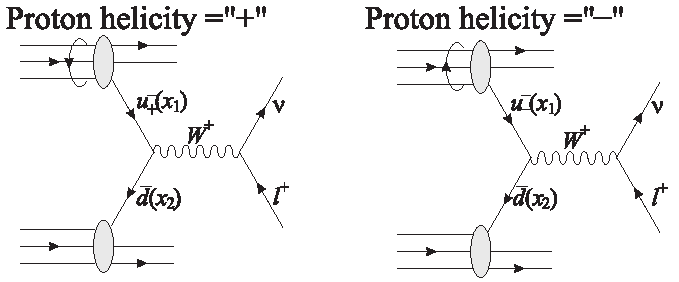
\includegraphics[width=0.8\linewidth]{./figures/w_plus_u_probe.pdf}
    \caption{
      Probe for $\Delta u$ at lowest order.
    }
    \label{fig:u_probe}
  \end{subfigure}
  \begin{subfigure}[t]{\textwidth}
    \centering
    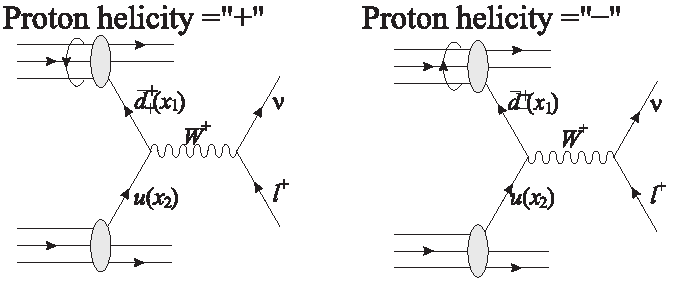
\includegraphics[width=0.8\linewidth]{./figures/w_plus_dbar_probe.pdf}
    \caption{
      Probe for $\Delta\bar{d}$ at lowest order
    }
    \label{fig:dbar_probe}
  \end{subfigure}
  \caption{
    Real $W^+$ production as produced at PHENIX. The helicity of the initial
    state fixes the helicity of the partonic participants due to the
    relativistic final state of the neutrino + the handedness of the W boson.
    $x_1$ and $x_2$ are the momentum fractions of the quarks participating from
    the participant partons~\cite{Aidala2005}. 
  }
  \label{fig:w_probe_leading_order}
\end{figure}

Though both protons in the collision are polarized, the polarization of one
participant proton can be effectively ignored by summing over all polarization
states for one of the two protons. With this assumption, we may construct a
single spin asymmetry for colliding protons by counting difference in the number
of positively and negatively polarized W's produced in collisions, scaled by the
total production:

\begin{equation}
  {{A_L}^W} =
  {{{1}\over{P}}\times{{N_{-}(W)-N_{+}(W)}\over{{N_{-}(W)+N_{+}(W)}}} }
  \label{eq:w_production_asymmetry}
\end{equation}

This is a relatively easy experimental probe to measure (assuming that we can
accurately count events which produced a W, which naturally, is nearly
impossible, as we will see in Section~\ref{sec:sbr}).

As we saw earlier, in Section~\ref{sec:polarized_pdfs}, we can write an
asymmetry in terms of the scattering cross section for the process responsible
for particle yields. These cross-sections were shown to be written in terms of
polarized parton distribution functions, thus, we cut to the chase to write down
the full expression of the theoretical asymmetries for this process in terms of
those parton distribution functions.

The following equations all contain an implied integration over $x_1$ and $x_2$.

For $W^+$ and $u$:
\begin{equation}
  {A_L^{W^+}} = 
  {
    {u_-^-(x_1)\bar{d}(x_2)-u_+^-(x_1)\bar{d}(x_2)}
    \over
    {u_-^-(x_1)\bar{d}(x_2)-u_+^-(x_1)\bar{d}(x_2)}
  }  
  \label{eq:al_u_full}
\end{equation}

For $W^+$ and $\bar{d}$
\begin{equation}
  {A_L^{W^+}} = 
  {
    {\bar{d}_-^+(x_1)u(x_2)-\bar{d}_+^+(x_1)u(x_2)}
    \over
    {\bar{d}_-^+(x_1)u(x_2)+\bar{d}_+^+(x_1)u(x_2)}
  }  
  \label{eq:al_dbar_full}
\end{equation}

Observationally, we see a superposition of \ref{eq:al_u_full} and
\ref{eq:al_dbar_full}, which is expressed in
Equation~\ref{eq:al_superposition_pos}:

\begin{equation}
  {A_L^{W^+}} = 
  {
    {
      \Delta u(x_1)\bar{d}(x_2)-\Delta \bar{d}(x_1)u(x_2)
    }
    \over
    {
      u(x_1)\bar d(x_2)+\bar(d)(x_1)u(x_2)
    }
  }
  \label{eq:al_superposition_pos}
\end{equation}

For the case of $W^-$, we observe $\bar{d}$ and $u$:
For $W^-$ and $d$:
\begin{equation}
  {A_L^{W^+}} = 
  {
    {d_-^-(x_1)\bar{u}(x_2)-d_+^-(x_1)\bar{u}(x_2)}
    \over
    {d_-^-(x_1)\bar{u}(x_2)-d_+^-(x_1)\bar{u}(x_2)}
  }  
  \label{eq:al_d_full}
\end{equation}

For $W^-$ and $\bar{u}$
\begin{equation}
  {A_L^{W^+}} = 
  {
    {\bar{u}_-^+(x_1)d(x_2)-\bar{u}_+^+(x_1)d(x_2)}
    \over
    {\bar{u}_-^+(x_1)d(x_2)+\bar{u}_+^+(x_1)d(x_2)}
  }  
  \label{eq:al_ubar_full}
\end{equation}

Observationally, we see a superposition of \ref{eq:al_d_full} and
\ref{eq:al_ubar_full}, which is expressed in
Equation~\ref{eq:al_superposition_neg}:

\begin{equation}
  {A_L^{W^-}} = 
  {
    {
      \Delta d(x_1)\bar{u}(x_2)-\Delta \bar{u}(x_1)d(x_2)
    }
    \over
    {
      d(x_1)\bar u(x_2)+\bar(u)(x_1)d(x_2)
    }
  }
  \label{eq:al_superposition_neg}
\end{equation}

Kinematics of the collision can simplify the equations even further, when at
very forward or very backward rapidities~\cite{Aidala2005}. Concretely, this is
shown via integration over the momentum fractions, $x_1$ and $x_2$, explicitly
writing the W decay in terms of the scattering cross section for polarized
proton collisions (a derivation reproduced from Hideyuki Oide's
thesis~\cite{Oide2012}):

\begin{multline}
  {
    d\sigma
    \left(
      p^{\Rightarrow}+p\rightarrow W^+\rightarrow \ell+\nu_{\ell}
    \right)
  } 
  = \\
  {
    {K\over3}\int dx_1dx_2\sum_{i,j}
    \left(
    q_{i-}^\Rightarrow(x_1)\bar{q}_{j+}(x_2) +
    \bar{q}_{j+}^\Rightarrow(x_1)q_{i-}(x_2)
    \right)
  }  \\
  \times
  {
    d\hat{\sigma}(q_i+\bar{q}_j\rightarrow W^+\rightarrow \ell^+ + \nu_{\ell})
  }
\end{multline}

{\noindent}Similarly, we may write the interaction cross-section for the
opposite helicity in the initial state:

\begin{multline}
  {
    d\sigma
    \left(
      p^{\Leftarrow}+p\rightarrow W^+\rightarrow \ell+\nu_{\ell}
    \right)
  } 
  = \\
  {
    {K\over3}\int dx_1dx_2\sum_{i,j}
    \left(
    q_{i-}^\Leftarrow(x_1)\bar{q}_{j+}(x_2) +
    \bar{q}_{j+}^\Leftarrow(x_1)q_{i-}(x_2)
    \right)
  }  \\
  \times
  {
    d\hat{\sigma}(q_i+\bar{q}_j\rightarrow W^+\rightarrow \ell^+ + \nu_{\ell})
  }
\end{multline}

Neglecting quark mass, we can assume that the helicity state of the quarks is
identical to the chirality state. Then, we substitute in the definition for
polarized parton distribution functions $\Delta q \equiv q_{+}^{\Rightarrow} -
q_{-}^{\Rightarrow}$, and sum over quark flavors, neglecting strange
contributions:

\begin{align}\label{eq:al_theory_quarks}
  {
    A_L
    \left(
      p^{\Rightarrow}+p\rightarrow W^+ \rightarrow \ell^+ +\nu_{\ell}
    \right)
  } &=  
  {
    {
      \int dx_1 dx_2 \sum_{i,j}
      \left(
        -\Delta q_i(x_1)\bar{q}_j(x_2)
        +\Delta \bar{q}_j(x_1)q_i(x_2)
      \right)\cdot d \hat{\sigma}
    }
    \over
    {
      \int dx_1 dx_2
      \sum_{i,j}(q_i(x_1)\bar{q}_j(x_2)+\bar{q}_j(x_1)q_i(x_2))\cdot d\hat{\sigma}
    }
 }\\
 & \approx  \nonumber
 {
   {
      \int dx_1 dx_2 
      \left(
        -\Delta u(x_1)\bar{d}(x_2)
        +\Delta \bar{d}(x_1)u(x_2)
      \right)\cdot d \hat{\sigma}
   }
   \over
   {
      \int dx_1 dx_2 (u(x_1)\bar{d}(x_2)+\bar{d}_j(x_1)u(x_2))\cdot d\hat{\sigma}
   }
 }
\end{align}

Since we have restricted ourselves to only the case for $u\bar{d}$, we are of
course looking at the case of $A_L^{W+}$. We may rewrite
Equation~\ref{eq:al_theory_quarks} to reflect its rapidity dependance:

\begin{equation}
  {A_L^{W+}(y_{\ell})} = 
  {
    {
     \int dx_1 dx_2 
     \left(
       -\Delta u(x_1)\bar{d}(x_2)(1-cos\hat{\theta})^2
       +\Delta \bar{d}(x_1)u(x_2)(1+cos\hat{\theta})^2
     \right)
    }
    \over
    {
       \int dx_1 dx_2 
       \left(
       (u(x_1)\bar{d}(x_2)   (1-cos\hat{\theta})^2
      +\bar{d}_j(x_1)u(x_2)) (1+cos\hat{\theta})^2
        \right)
    }
  }
  \label{eq:al_w_pos_rapidity_dependance}
\end{equation}

In this case, we follow Dr. Oide's convention of redefining $\hat{\theta}$ in
terms of the angle between the direcion of momentum of the polarized proton and
the leptop in the center of mass frame. Therefore we see kinematic isolation of
the polarized pdfs at forward or backward rapdity.\\

{\noindent}We may write $A_L^{W-}(y_{\ell})$ similarly:

\begin{equation}
  {A_L^{W-}(y_{\ell})} = 
  {
    {
     \int dx_1 dx_2 
     \left(
       -\Delta \bar{u}(x_1)d(x_2)(1-cos\hat{\theta})^2
       +\Delta d(x_1)\bar{u}(x_2)(1+cos\hat{\theta})^2
     \right)
    }
    \over
    {
       \int dx_1 dx_2 
       \left(
         (\bar{u}(x_1)d(x_2)   (1-cos\hat{\theta})^2
         +d_j(x_1)\bar{u}(x_2)) (1+cos\hat{\theta})^2
        \right)
    }
  }
  \label{eq:al_w_neg_rapidity_dependance}
\end{equation}
\clearpage
\section{Cross Sections and Luminosity}
\begin{itemize}
		\item vernier analysis note intro, equations
		\item summarize the papers on Lumoninosity
\end{itemize}

\textbf{Questions I'd Like to Answer in this Chapter}
\begin{enumerate}
    \item Why can we collide two polarized protons, but pretend that only one of
      them is polarized? What if summing over polarization states doesn't
      'cancel' this out?
    \item Why is $A_L$ an appropriate probe for proton spin
    \item How exactly do we go from a measurement of $A_L$ to an understanding
      of proton spin?
    \item Why do we need to calculate $A_{LL}$? What does it tell us? Why do we
      combine the helicities in the way we do, to define $A_{LL}$?
\end{enumerate}

Double spin asymmetry:

\begin{equation}
  A_{LL} = {
    {d\sigma^{\Rightarrow\Rightarrow}-d\sigma^{\Leftarrow\Rightarrow}}
    \over
    {d\sigma^{\Rightarrow\Rightarrow}+d\sigma^{\Leftarrow\Rightarrow}}
  }
\end{equation}
\clearpage
